\section{Задание 3 --- обмен информацией с Web-сервером}

Создайте веб-приложение, которое формирует возрастающую последовательность из чисел, переданных через поля ввода формы.

Ввод данных:

\begin{center}
  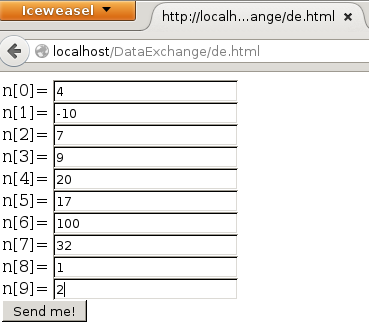
\includegraphics[width=9cm]{img/09.png}
\end{center}

Результат:

\begin{center}
  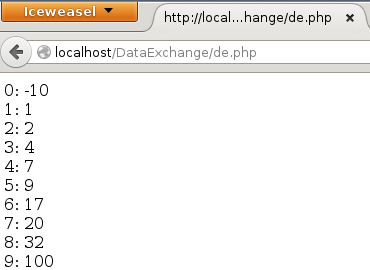
\includegraphics[width=9cm]{img/10.png}
\end{center}

Исходный код \verb|de.html|:

\begin{verbatim}
<form action="de.php" method="post">
  n[0]=  <input type="text" name="n0" /><br />
  n[1]=  <input type="text" name="n1" /><br />
  n[2]=  <input type="text" name="n2" /><br />
  n[3]=  <input type="text" name="n3" /><br />
  n[4]=  <input type="text" name="n4" /><br />
  n[5]=  <input type="text" name="n5" /><br />
  n[6]=  <input type="text" name="n6" /><br />
  n[7]=  <input type="text" name="n7" /><br />
  n[8]=  <input type="text" name="n8" /><br />
  n[9]=  <input type="text" name="n9" /><br />
  <input type="submit" name="submit" value="Send me!" />
</form>
\end{verbatim}

Исходный код \verb|de.php|:

\begin{verbatim}
<?php
$myArray = array();

//Грузим данные в массив
for ($i = 0; $i < 10; $i = $i + 1){
    $myArray[$i] = $_POST["n{$i}"];
}

// Сортируем массив
for ($i = 0; $i < 9; $i = $i + 1){
    $minIndex = $i;
    for ($j = $i + 1; $j < 10; $j = $j + 1){
        if ($myArray[$j] < $myArray[$minIndex]) $minIndex = $j;
    }
    $temp = $myArray[$i];
    $myArray[$i] = $myArray[$minIndex];
    $myArray[$minIndex] = $temp;
}

// Вывод массива на страницу
for ($i = 0; $i < 10; $i = $i + 1){
    echo "{$i}: {$myArray[$i]} <br>";
}
?>
\end{verbatim}
